\chapter{Podwarstwa Medium Access Control}
\label{cha:mac}

Podwarstwa MAC (Medium Access Control) jest trzecią z podwarstw warstwy Access Stratum. Z podwarstwą RLC komunikuje się ona za pośrednictwem kanałów logicznych (logical channels) i wymienia z nią jednostki danych (SDU). Natomiast z warstwą fizyczną (PHY) komunikuje się przy użyciu kanałów transportowych (transport channels) i odbiera oraz przekazuje do niej dane w formie bloków transportowych.

\begin{figure}
	\centerline{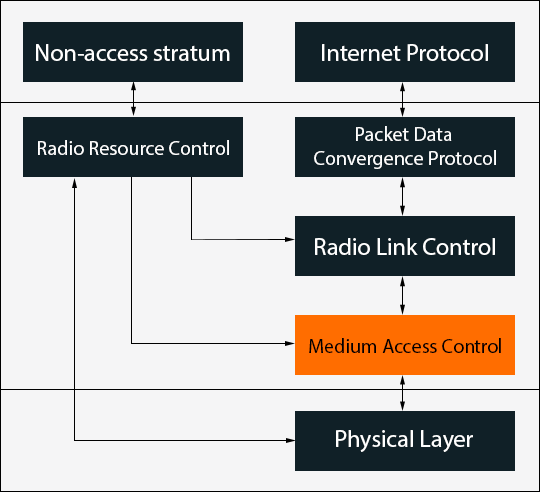
\includegraphics[width=0.4\textwidth]{images/mac_overview.png}}
	\caption{Umiejscowienie podwarstwy MAC w stosie protokołów LTE}
	\label{fig:mac_overview}
\end{figure}

Do funkcji podwarstwy MAC możemy zaliczyć:

\begin{enumerate} 
	\item Mapowanie jednostek danych (SDU) przesyłanych do kanałów logicznych na kanały transportowe gdzie formowane są w bloku tranportowe zawierające PDU
	\item Planowanie jak i kiedy jednostki danych mają zostać dostarczone
	\item Swobodny dostęp
	\item Zarządzenie synchronizacją czasu pomiędzy urządzeniem użytkownika a stacją bazową 
\end{enumerate}


\section{Mapowanie kanałów}

Podwarstwa MAC komunikuje się z podwarstwą RLC za pośrednictwem kanałów logicznych. Można je podzielić na kanały ``control channels`` transportujące dane dotyczące ``control plane`` oraz na kanały ''traffic channels'' transportujące dane dotyczące ''control plane''.

Wyróżniamy następujące kanały logiczne typu ``control channels``:

\begin{enumerate}
	\item Broadcast Control Channel (BCCH)
	\item Paging Control Channel (PCCH)
	\item Common Control Channel (CCCH)
	\item Multicast Control Channel (MCCH)
	\item Dedicated Control Channel (DCCH)
\end{enumerate}

Kanały logiczne typu ``traffic channels`` są następujące:

\begin{enumerate}
	\item Dedicated Traffic Channel (DTCH)
	\item Multicast Traffic Channel (MTCH)
\end{enumerate}

Z warstwą fizyczną (PHY), podwarstwa MAC komunikuje się przy użyciu kanałów transportowych ``transport channels``. Dzielimy na kanały, ktore wysyłają dane od stacji bazowej do urządzenia użytkownika tzw. ``downlink channels`` oraz kanały używane do wysyłania danych od urządzenia użytkownika do stacji bazowej ``uplink channels``.

Wyrózniamy następujące ``downlink channels``:

\begin{enumerate}
	\item Broadcast Channel (BCH)
	\item Downlink Shared Channel (DL-SCH)
	\item Paging Channel (PCH)
	\item Multicast Channel (MCH)
\end{enumerate}

Oraz następujące ``uplink channels``:

\begin{enumerate}
	\item Uplink Shared Channel (UL-SCH)
	\item Random Access Channel (RACH)
\end{enumerate}

\begin{figure}
	\centerline{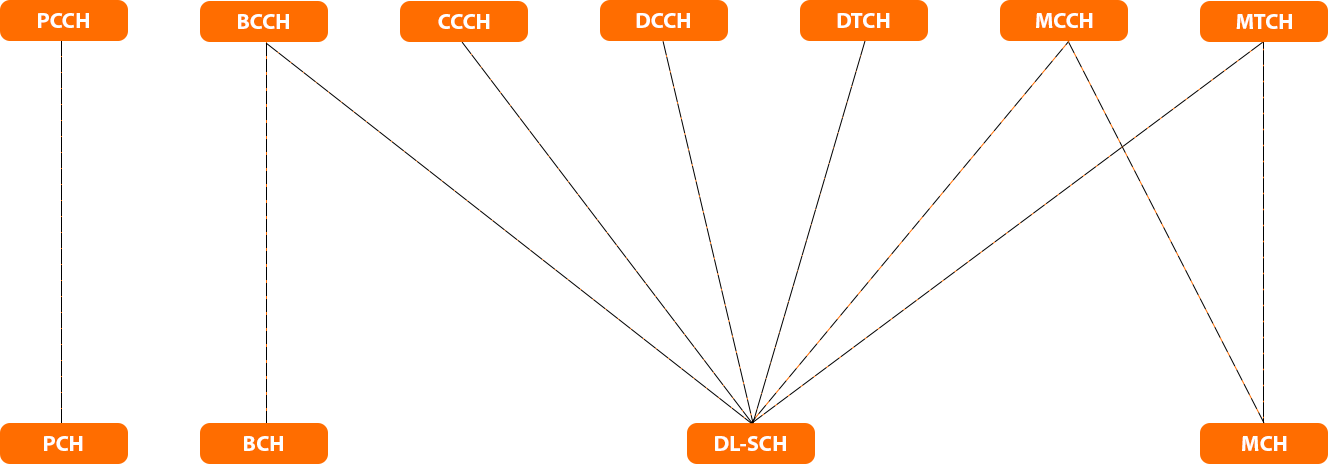
\includegraphics[width=0.8\textwidth]{images/mac_downlink_mapping.png}}
	\caption{Mapowanie kanałów logicznych na kanały transportowe dla downlink channels}
	\label{fig:mac_downlink_mapping}
\end{figure}

\begin{figure}
	\centerline{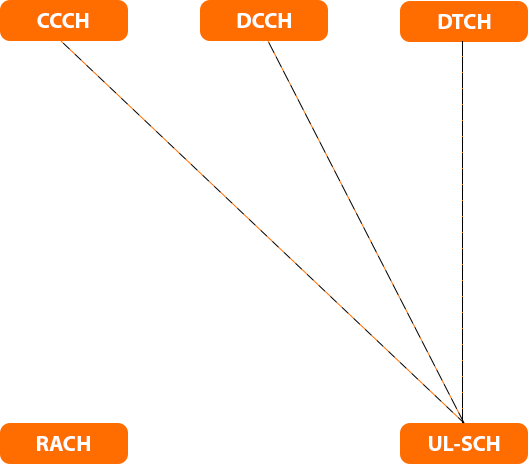
\includegraphics[width=0.5\textwidth]{images/mac_uplink_mapping.png}}
	\caption{Mapowanie kanałów logicznych na kanały transportowe dla uplink channels}
	\label{fig:mac_uplink_mapping}
\end{figure}

\section{Korekcja błędów HARQ}

\section{DRX}

\section{Struktura pakietów}
